\chapter{Introduction}

\gls{co2} is the primary greenhouse gas emitted through human activity \cite{Emissions_2023}. Higher levels of \gls{co2} in the atmosphere can lead to further heat retention, causing global temperature levels to rise at a record-breaking rate \cite{Lindsey_2023,}. In an effort to reduce man-made contributions toward issues related to climate change, carbon capture and sequestration has become a prominent area of research \cite{}. A natural extension of this line of research might then be to ask: what does one do with all of this collected \gls{co2}? Are there industrial or technological applications that can benefit from this available reserve? Luckily, the answer to that question is a resounding ``yes''.

%Fluids are a vital part of everyday life - two of the most common ones being the air we breath and the water we drink. Less obvious are all the ways even these common fluids function behind the scenes in our day to day activities. Water, for example, serves an important role in various industrial settings, proving useful in areas ranging from thermal management to energy production; steam turbines alone accounted for 45\% of electricity generation in the United States in 2021 \cite{US_elec_gen_stat}. Improvements to these types of systems impact technologies across a variety of fields and are thus an important area of research \cite{}. One strategy toward this end, and the primary motivator of the research presented here, is the use of supercritical fluids as the working fluid of these systems. 

The applications used to motivate this research are all concerned with supercritical Carbon Dioxide (sCO2), in particular. \gls{sco2} has many beneficial features that are important to a wide variety of industrial applications, as we will detail further later on in this chapter. Many of these applications of interest include injection technologies that involve a round turbulent jet configuration within the system. Much research has gone into supercritical jet turbulence, however, due to extreme thermodynamic variation around the supercritical point (a region known as the pseudo-critical zone), slight changes in parameter regime result in significant changes in flow dynamics \cite{}. Thus there is much research needed still in order to fully understand the fundamental flow physics within this area of interest. 

The goal of this work is to further explore the pseudo-boiling region of the pseudo-critical zone and analyze the influence of extreme thermodynamic fluctuations on turbulence statistics and flow dynamics within the flow field. To that end, the rest of this chapter continues as follows: first, we cover important definitions relating to fluids in order to establish what a supercritical fluid even is. Then, the mathematical framework for modeling compressible Newtonian fluids is provided to form the basis of the modeling done in this dissertation. Further consideration is then given to turbulence modeling and the numerical methods developed for studying turbulence to provide insight into the quantities of interest analyzed within this dissertation and the choices of numerical methods used herein. Important applications of supercritical carbon dioxide in particular are provided to motivate the problem presented in this dissertation. Existing numerical studies on supercritical fluids are reviewed to demonstrate how this dissertation fits into the current landscape of research and to emphasize the contribution the results of this work make to the field. This chapter concludes with an outline of the dissertation, the goals of the dissertation, and the main contributions made through this work. 

\section{What is a Fluid?} 

In order to discuss supercritical fluids further, we must first go into more detail about general fluids. Here we go over the general definitions and distinctions given to fluids as outlined by Batchelor \cite{batchelor_2000}. One of the defining characteristics that can be used to distinguish fluids from solids is the ease with which they deform. Generally, a solid material has a definite shape and internal structure, which only changes when acted upon by external forces. Fluids on the other hand do not have a preferred shape. More specifically, elements within a parcel of fluid can experience rearrangement through chaotic motion without affecting the macroscopic nature of the parcel. This continuous and relatively large deformation given a potentially small but suitable external force is one way to distinguish a fluid from a solid, where instead small external force only results in small internal change. 

The two categories of fluids that most people are familiar with are gases and liquids. These two states are mainly distinguished by differences in intermolecular scales and forces. Molecules within a gas are, on average, much farther apart than they are in liquids. This separation is so vast in gases, that molecules only experience very weak cohesive forces, except for when the rare collision occurs \cite{batchelor_2000}. Molecules within liquids, on the other hand, are close enough to affect one another through near-field attractive forces at any given time. A simplified distinction between the two is that both gases and liquids will conform to the shape of whatever container they are in, but gases will further spread to fill all available space present. 

The state of a fluid can be uniquely determined by two quantities: pressure and density. Pressure is the force per unit area exerted by the fluid on its boundaries \cite{PAINE19941-1}. Density is the mass per unit volume of the fluid \cite{PAINE19941-1}. These two quantities can be related to other important information, like temperature, which indicates the level of thermal energy in the fluid \cite{PAINE19941-1}. In gases, the main contribution to pressure is the force normal to the surface of each individual molecule on the fluid boundary. Reducing the volume of a fixed mass of gas while maintaining a constant temperature will increase the density, thus reducing the average distance between molecules. If, however, this distance remains relatively large compared to the size of the molecule, then intermolecular forces are still negligent and do not significantly contribute to pressure. Fluids that allow for this reduction are said to be compressible. By contrast, molecules within liquids experience strong cohesive forces due to their close proximity to one another \cite{batchelor_2000}. If density is increased even slightly at constant temperature, the pressure contribution experienced toward one molecule by its neighbors greatly increases, resulting in a large pressure change. Fluids that show a resistance to this volume reduction process are then said to be incompressible. In either case, the relationship between pressure, temperature, and density can be measured and modeled through mathematics, as we will see later on in this chapter. 

\subsection{Supercritical Fluids}

A supercritical fluid is a fluid that is held above a critical temperature and pressure, at which point the distinction between a gas and liquid phase no longer exists \cite{SCF2, SCF1}. Supercritical fluids have qualities associated with both gases and liquids yet simultaneously have features that exclude them from fully being categorized as one or the other. For example, while they have viscosities akin to gases, they have solvent capabilities associated with liquids \cite{}. Similarly, while they have densities in line with liquids, they lack surface tension \cite{}. One benefit of this duality is that supercritical fluids can be fine tuned to be more gas-like or more liquid-like depending on the application at hand. This also results in ambiguity on how to actually classify them, with some sources considering them highly compressed gases \cite{Gordon}, expanded liquids \cite{Aggarwal}, or even as their own distinctly separate phase \cite{BANUTI201512}. The distinction usually lies on the specifics of the regime and the application at hand. 

We focus on one particular fluid of interest: \gls{co2}. As seen in the phase diagram of Figure \ref{phase_diagram}, the critical temperature, $T_c$, and critical pressure, $p_c$, of \gls{co2} are $304.128 $ K and $73.773$ bar. The critical temperature and pressure of \gls{co2} is fairly easy to attain, making it a strong candidate for systems with hight thermal outputs. Additionally, \gls{sco2} has a relatively low toxicity and environmental impact \cite{}, and is chemically stable, non-flammable, and readily available \cite{}. For these reasons, \gls{sco2} is a highly coveted alternative working fluid in many different applications, and is one of the most widely used supercritical fluids along with water \cite{SCF2}. 

\begin{figure}[h!]
\begin{center}
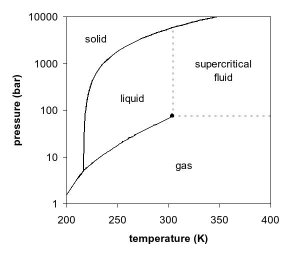
\includegraphics[scale=.75]{figures/co2_phase_diagram}
\end{center}
\caption{Phase diagram for Carbon Dioxide (CO2). Critical pressure, $p_c$, and temperature, $T_c$, are $73.773$ bar and $304.128$ K, respectively.}
\label{phase_diagram}
\end{figure}

In the next part of this section, we will explore some applications of \gls{sco2} where the turbulent round jet configuration is used in order to further motivate the investigation outlined in this work. 

\subsection{Applications of Interest}
One of the key applications of interest that motivates this work is the use of \gls{sco2} as the working fluid in advanced cycles for power generation. \gls{sco2} has shown promise as a working fluid for both indirect cycle and direct-firing cycles \cite{WEILAND2017293, WHITE2021116447}. One example of indirect cycle improvement uses \gls{sco2} in place of water for the conventional steam-Rankine cycle. An example of where these types of configurations may prove useful is in managing thermal runoff from existing coal and natural gas combustion processes \cite{WEILAND2017293}. Compared to steam, \gls{sco2} is less corrosive, more thermally stable, and has increased power density. The critical point of \gls{co2} is easily accessible, and once achieved, allows for the use of a single phase fluid design, leading to a simplified and more compact turbine (see Figure \ref{turbine_comp}). Ultimately, this also allows for lower operation and maintenance costs \cite{Dodge}. The benefits of using sCO2 turbines over the traditional steam design has been highly researched and has only seen an increase in momentum for implementation \cite{CRESPI2017152, NextGenNucReac, Dodge, commercialization}. 

\begin{figure}[h!]
\begin{center}

\includegraphics[scale=.5]{figures/steam_vs_sco2_turbine}
\end{center}
\caption{Size comparison for steam vs. \gls{sco2} turbine via Echogen Power Systems LLC \cite{commercialization}.}
\label{turbine_comp}
\end{figure}

An example of direct-firing cycles that use \gls{sco2} include the Allam cycle \cite{allam2013system}. When compared to the conventional Brayton cycle, studies show that the Allam cycle has much higher efficiency \cite{ALLAMCOMP, ALLAM20175948}. Additionally, the carbon footprint for the Allam cycle is virtually zero, allowing for \gls{co2} produced from the system to be stored underground or used elsewhere, aiding in carbon sequestration efforts \cite{cleantechnol1010022}. This two-for-one benefit of using \gls{sco2}-based cycles such as the Allam cycle has spurned much research \cite{ALLAMTech1, CHAN2021113972} and development \cite{8Rivers} into related technologies.

Of particular importance to these applications is the round turbulent jet, as this is a major component of many injection technologies. The high densities associated with the liquid-like aspect of supercritical fluids coupled with the relatively low gas-like viscosity associated with them typically results in a high Reynolds flow, often resulting in a turbulent system. The turbulence physics of these jets is crucial in developing machinery for these systems. 

\section{Mathematics of Fluid Flow}

Scale is one of the key factors to consider when developing a mathematical description of a fluid system. For example, consider modeling flow past a satellite in the exosphere vs. the flow past a turtle in the ocean; these two mediums have vastly different characteristics and would thus require different modeling techniques. Scale is also an important concept when it comes to turbulence in particular so we will begin that discussion here with our choice in perspective for the mathematical framework of our system of interest.

From a kinetics perspective, particle motion within a fluid can be broken up into two phases: particle interaction and free flight. Average time spent in free flight, $<t_f>$, is typically much greater than collision time for a given interaction, $t_c$. The average length traveled between collisions is known as the mean free path, $\ell$.  Since free flight time dominates particle interaction time, this phase determines the length scale of the kinetic description of motion. In addition to this inherent physical scale, there is also a scale associated with the resolution of the problem itself, $L$. These two scales are important, as the mathematical description of your model depends on how these two scales compare to one another. This comparison is related through the non-dimensional Knudsen number: 
\begin{equation}\label{Knudsen}
Kn = \dfrac{\ell}{L}
\end{equation} 
Flows with large Knudsen number ($Kn \gg 10$) require modeling from the kinetic or microscopic perspective as particle interactions become sparse enough compared to the scope of the problem to require a statistical mechanics framework. On the other hand, small Knudsen number flows ($Kn \ll 0.01$) have a problem scale that far exceeds the particle-level interactions present, giving way to an average overall motion within the fluid. This scale dichotomy is demonstrated with the graphic in Figure \ref{Knudsen}. For small Knudsen flows, a continuum description of the fluid is appropriate for capturing this macroscopic behavior. 

\begin{figure}[h!]
\begin{center}
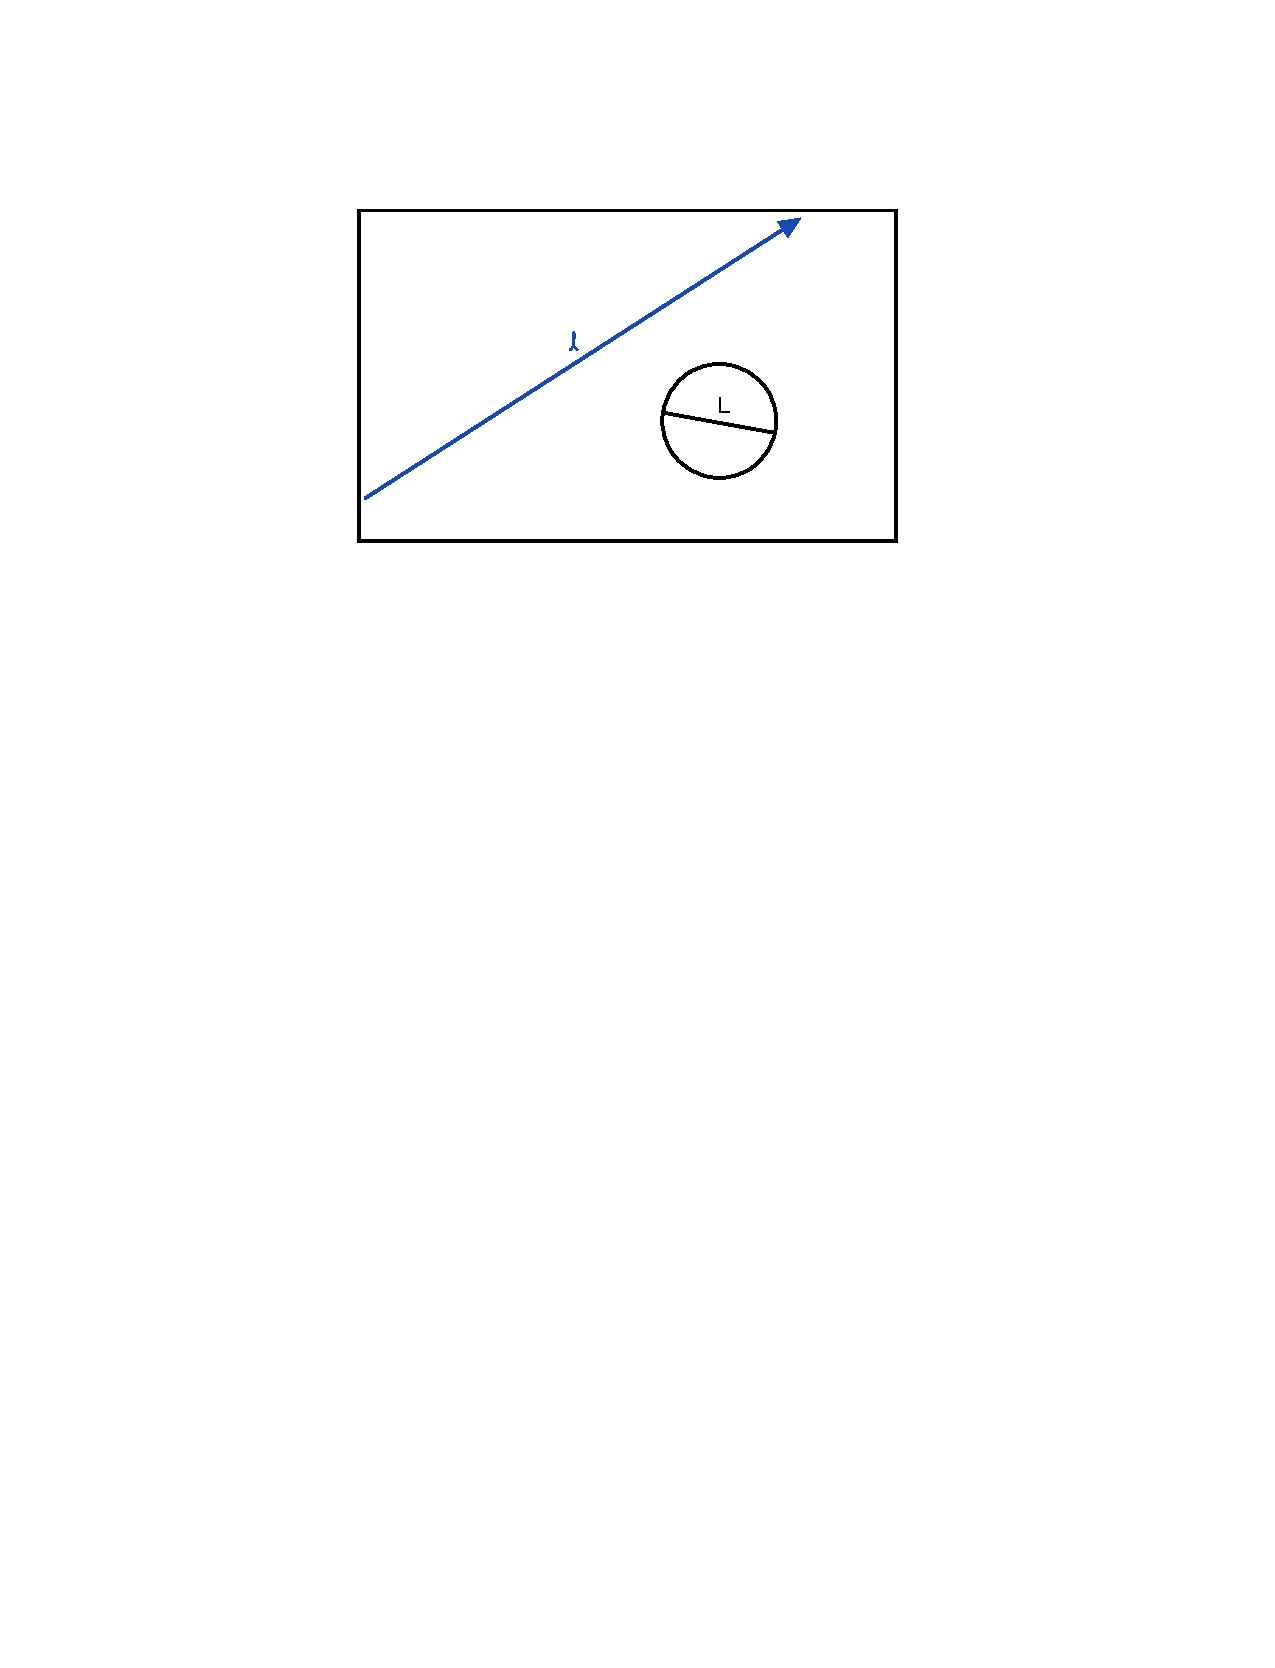
\includegraphics[scale=0.6]{figures/Large_Kn.pdf}
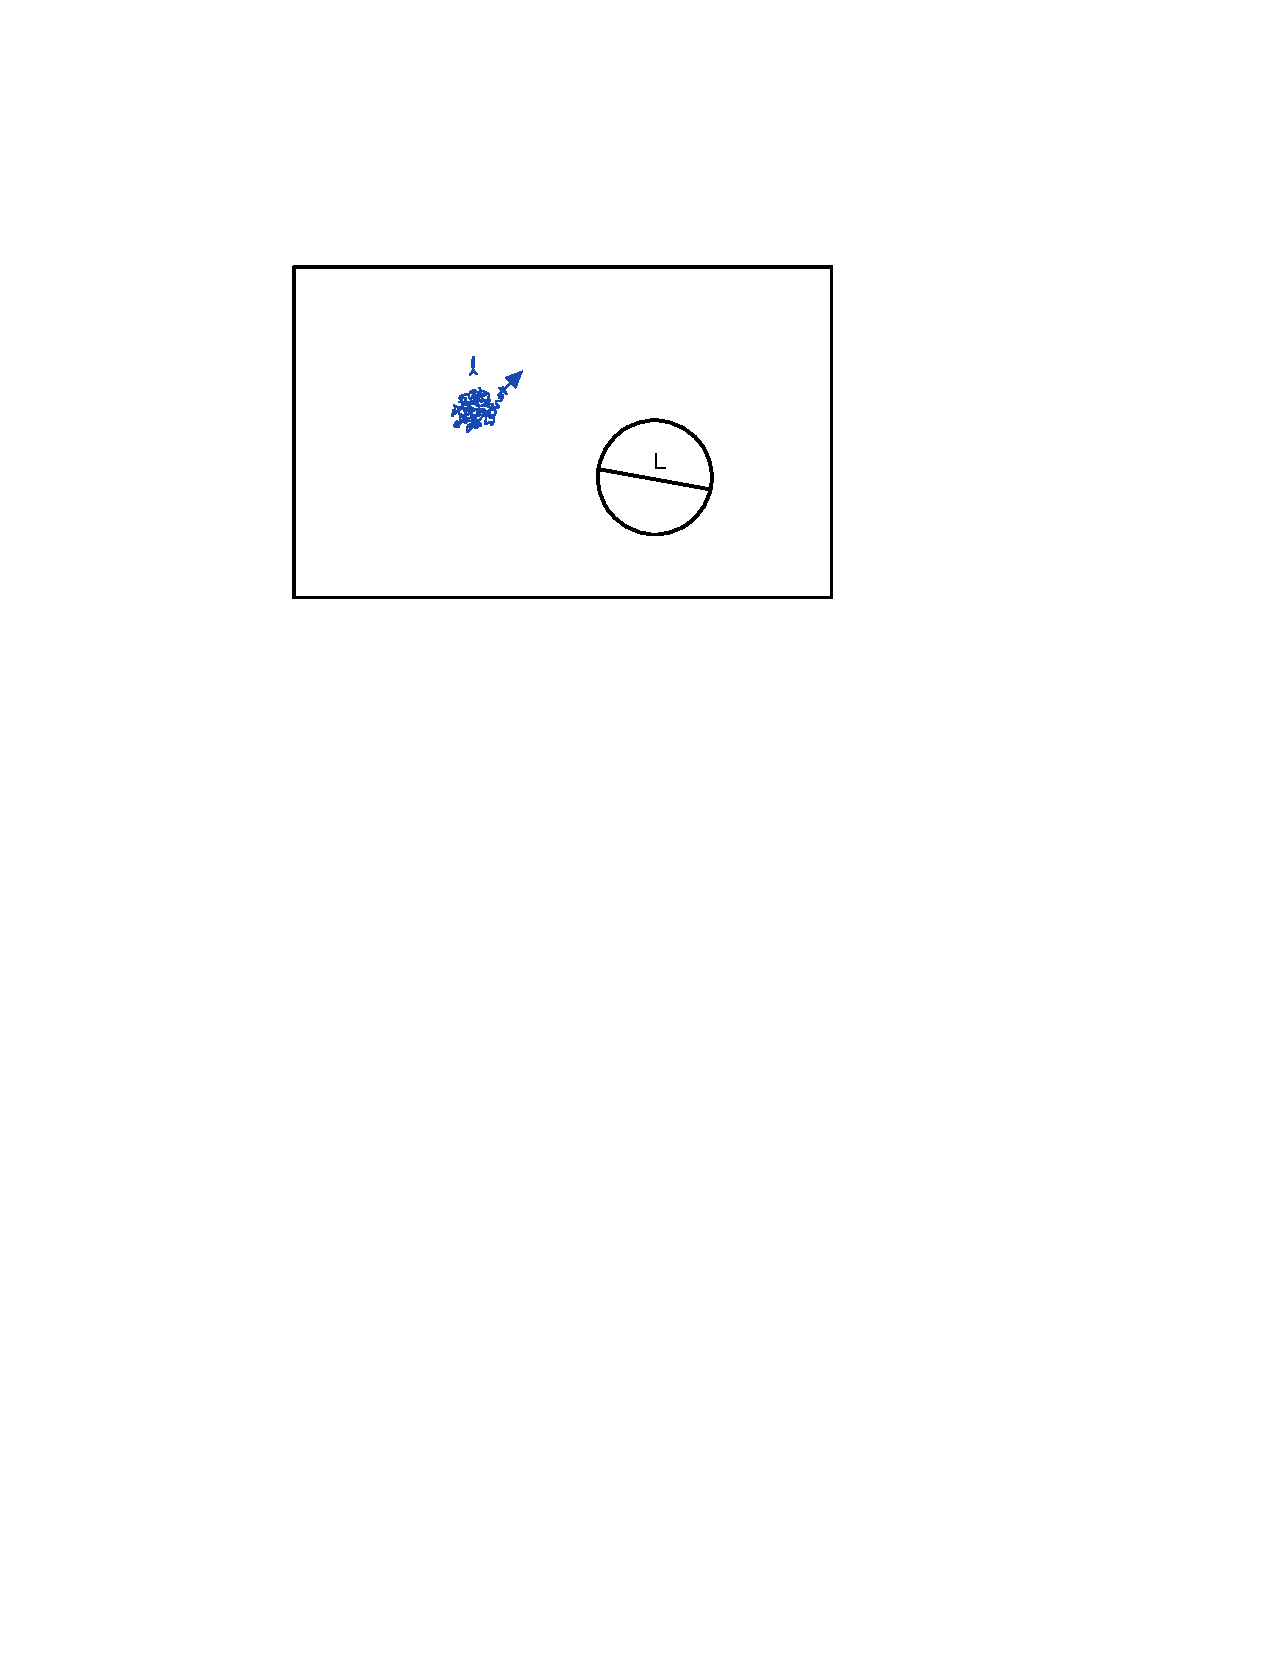
\includegraphics[scale=0.6]{figures/Small_Kn.pdf}
\end{center}
\caption{Characteristic length scale of problem, $L$, compared to mean free path of particles, $\ell$, for a flow with large Knudsen number (left) vs. small Knudsen number (right)}
\label{Knudsen_example}
\end{figure}

This work falls within the small Knudsen regime, so we will be working with the continuum description of fluids. In this section we will discuss the Navier-Stokes Equations that arise from this modeling technique and how we account for the supercritical nature of the flow through our choice of equation of state. 

\subsection{Continuum Description of Fluids}
The continuum hypothesis assumes that the fluid has no fine structures and that it is perfectly continuous, i.e., the properties of a small subdivision are the same as other subdivisions. This allows for the approximation of physical quantities at the infinitesimal limit \cite{cont}.

For example, consider a fluid with arbitrary volume $V$ as depicted in Figure \ref{cons_mass}.  

\begin{figure}[h!]
\begin{center}
\begin{tikzpicture}

% Blob
\path[draw, style=dashed, scale=1.5, use Hobby shortcut]
(1,.4) .. (.8, -.425) .. (1,-1.25);
\path[draw, style=dashed, scale=1.5, use Hobby shortcut]
(2,.77) .. (1.7, -.365) .. (2,-1.5);
\path[draw,scale=1.5, style=dashed, use Hobby shortcut]
(3,1) .. (2.6, -.185) .. (3,-1.37);

\path[draw, color=red, -stealth,scale=1.5, use Hobby shortcut, save Hobby path = {velocity}]
(-.5,-.125) .. (0,0) .. (1,-.25) .. (2,-.5) .. (3,-.25) .. (4, 0) .. (4.5, -.125);
\path[draw, color=red, yshift=1cm, -stealth,scale=1.5, use Hobby shortcut]
(-.5,-.125) [ restore and use Hobby path={velocity}{}];
\path[draw, color=red, yshift=-1cm, -stealth,scale=1.5, use Hobby shortcut]
(-.5,-.125) [ restore and use Hobby path={velocity}{}];

\path[draw, thick, scale=1.5, use Hobby shortcut, closed=true]
(0,0) .. (1,.4) .. (3,1) .. (4,.3) .. (2,-1.5) .. (.5,-1);
\path[draw,scale=1.5, use Hobby shortcut]
(1,.4) .. (1.2, -.425) .. (1,-1.25);
\path[draw,scale=1.5, use Hobby shortcut]
(2,.77) .. (2.3, -.365) .. (2,-1.5);
\path[draw,scale=1.5, use Hobby shortcut]
(3,1) .. (3.4, -.18) .. (3,-1.36);

\draw (-1.3, -.2) node[right][red]{v};
\draw (6, -2) node[right]{n};

\path[draw,scale=1.5, -stealth, use Hobby shortcut]
(3.6,-1) .. (4,-1.4);


\end{tikzpicture}
\end{center}
\caption{A fluid of arbitrary volume $V$ bounded by surface $S$ with velocity $\vb{v}(\vb{x},t)$. A differential volume and surface area is given by $dv$ and $ds$, respectively. $\vb{n}$ is the outward-pointing unit normal vector to the surface $S$.}
\label{cons_mass}
\end{figure}
For a fluid with density $\rho(\vb{x},t)$, mass within a small representative volume can be described with
$$ \rho \, dv$$
Total mass in the arbitrary volume is then given by 
$$\iiint_{V} \rho \,dv$$
The rate of change of mass through the volume is now 
$$\dfrac{d}{dt}\iiint_{V} \rho \, dv $$
\begin{equation} \label{volume_mass}
= \iiint_{V} \dfrac{\partial \rho}{\partial t}\,dv
\end{equation}
Simultaneously, overall change in mass throughout the volume can be described by the net mass flux through the surface $S$. Volumetric flow through a small portion of the bounding surface is given by
$$\vb{v}\cdot \vb{n} \, ds$$
Total mass flux through the entire surface is then
\begin{equation} \label{surface_flowthrough}
\iint_S \rho \, \vb{v}\cdot \vb{n} \, ds
\end{equation}
Applying the divergence theorem to Equation \eqref{surface_flowthrough} yields the following volume integral
\begin{equation} \label{volume_equiv}
\iiint_V \nabla \cdot \left(\rho \, \vb{v} \right) \, dv
\end{equation}
Assuming there is no additional source generating or leaking mass within the control volume, we can relate Equations \eqref{volume_mass} to \eqref{volume_equiv} : 
\begin{equation*}
\begin{aligned}
\iiint_{V} \dfrac{\partial \rho}{\partial t}\,dv &= - \iiint_V \nabla \cdot \left(\rho \, \vb{v} \right) \, dv \\ 
\iiint_{V} \dfrac{\partial \rho}{\partial t}\,dv &+ \iiint_V \nabla \cdot \left(\rho \, \vb{v} \right) \, dv  = 0 
\end{aligned}
\end{equation*}
\begin{equation} \label{cont_int}
\iiint_{V} \left( \dfrac{\partial \rho}{\partial t} + \nabla \cdot \left(\rho \, \vb{v} \right) \,\right) dv  = 0
\end{equation}
Note the inclusion of the negative sign for the right side of the initial equality; in the surface integral formulation, the outward facing normal describes flux out of the volume, thus yielding a decrease in mass within the volume. Since Equation \eqref{cont_int} holds for any arbitrary volume $V$, the integrand must be identically equal to zero:
\begin{equation} \label{conservation_mass}
\dfrac{\partial \rho}{\partial t} +  \nabla \cdot \left(\rho \, \vb{v} \right) \,  = 0
\end{equation}
Through the continuum hypothesis and conservation of mass, we have now arrived at the continuity equation in Equation \eqref{conservation_mass}. This specific process demonstrates an even more fundamental relationship known as a \textit{conservation law}. More generally, for some integrated property $\phi$, the rate of change of $\phi$ within a control volume must be equal to the amount of $\phi$ lost or gained through the boundaries of the control volume plus what is created or consumed by any sinks or sources, $s$, within the volume (sinks having positive orientation to match the positive orientation of the outward-facing normal $\vb{n}$) \cite{}. 
\begin{equation} \label{conservation_law}
\dfrac{\partial \phi}{\partial t} +  \nabla \cdot \left(\phi \, \vb{v} \right) + s \,  = 0
\end{equation}
In addition to this concept applying to conservation of mass, as was seen in this section, the idea outlined by Equation \eqref{conservation_law} applies to conservation of momentum and energy within the fluid. Together, these expressions combine to form the basis of the Navier-Stokes Equations, as will be seen in more detail in chapter 2. The important takeaway from this section is that with the continuum hypothesis and fundamental laws of physics, one can adequately capture macroscopic flow behavior for the types of flows we are interested in within this work.  

\subsection{Equation of State}
Conservation of mass, momentum, and energy gives us five equations to describe our fluid system. For compressible flows, this is not enough information to solve for all the unknowns within the system of coupled partial differential equations. A sixth equation, known as the \gls{eos}, must be chosen in order to close the system. The \gls{eos} relates three of the six unknowns: pressure, temperature, and density. Here we will briefly discuss some \gls{eos} options and their distinguishing characteristics in order to motivate the choice made for this work. 

The simplest option available is the ideal gas \gls{eos}, which comes from the ideal gas law. This \gls{eos} relates density, pressure, and temperature in the following manner: 
\begin{equation} \label{ideal_gas}
p = \dfrac{RT}{V_m}
\end{equation}
where $p$ is pressure, $R$ is the universal gas constant, $T$ is temperature, and $V_m = \tfrac{V}{n}$ is the molar volume of the fluid (it is common to express density in terms of molar volume for sake of simplicity in writing the \gls{eos} with $V$ being volume and $n$ being the number of moles). The ideal gas \gls{eos} is fairly accurate for liquids and gases at moderate temperatures and low pressures. It fails at low temperatures and high pressures, especially near the transition region from gas to liquid. The inaccuracy noted in this region means this \gls{eos} would not be suitable for the area of interest within this study. 

Cubic \gls{eos} generally provide more accuracy than the ideal gas \gls{eos}. The first cubic \gls{eos} was developed by van der Waal in 1873, modifying the ideal gas \gls{eos} to take into consideration the finite size of molecules and interactions between molecules (the ideal gas \gls{eos} only accounts for interactions with the container and treats molecules as point particles). Other cubic \gls{eos} can be thought of as modifications from this base form: 
\begin{equation} \label{vanderwaal}
p = \dfrac{RT}{V_m - b} - \dfrac{a}{V_m^2}
\end{equation}
where $a$ and $b$ are constants related to the pressure and temperature at the critical point, $p_c$ and $T_c$ respectively: 
$$a = \dfrac{27(RT_c)^2}{64p_c}\,, \quad b = \dfrac{RT_c}{8p_c}$$
One of the main benefits of using a cubic \gls{eos} is that they can have comparable and sometimes even better accuracy compared to their higher order counterparts, thus reducing computational costs. However, it is important to take into consideration the regime of interest in addition to the fluid of interest when choosing an \gls{eos}, as each one has its own pros and cons. For example, molecule polarity and density are two factors that can have a high impact in selection between the \gls{srk} and \gls{pr} alone \cite{GHANBARI201713}. 

This work uses the \gls{srk} as will be more thoroughly introduced in chapter 2. It has been shown that this equation of state is fairly accurate for the parameter regime under careful consideration in this work \cite{}. This accuracy is detailed further in chapter 3 through comparisons with data from \gls{nist}. Overall, when adequately considered, the \gls{eos} is the key avenue to incorporating specific fluid properties into the mathematical model.


\section{Turbulence}
In addition to categorizing by fluid type, fluid flow can be categorized based on flow characteristics. The main two classifications of note are laminar flow and turbulent flow.

Laminar flow is denoted by fluid particles having well-defined parallel trajectories of motion, or streamlines. Streamlines do not cross, meaning adjacent layers within the fluid flow by one another with little to no mixing. From a more generalized perspective, the flow appears to be smooth. In contrast to this, turbulent flow is characterized by its unpredictable and chaotic trajectories. Streamlines do cross resulting in swirls and eddies of varying length scales which induce mixing. Turbulent flow can be qualitatively described as being rough due to this high degree of fluctuation within the velocity and pressure fields present. This generalized description is depicted in Figure \ref{lam_vs_turb}.

\begin{figure}[h!]
\begin{center}
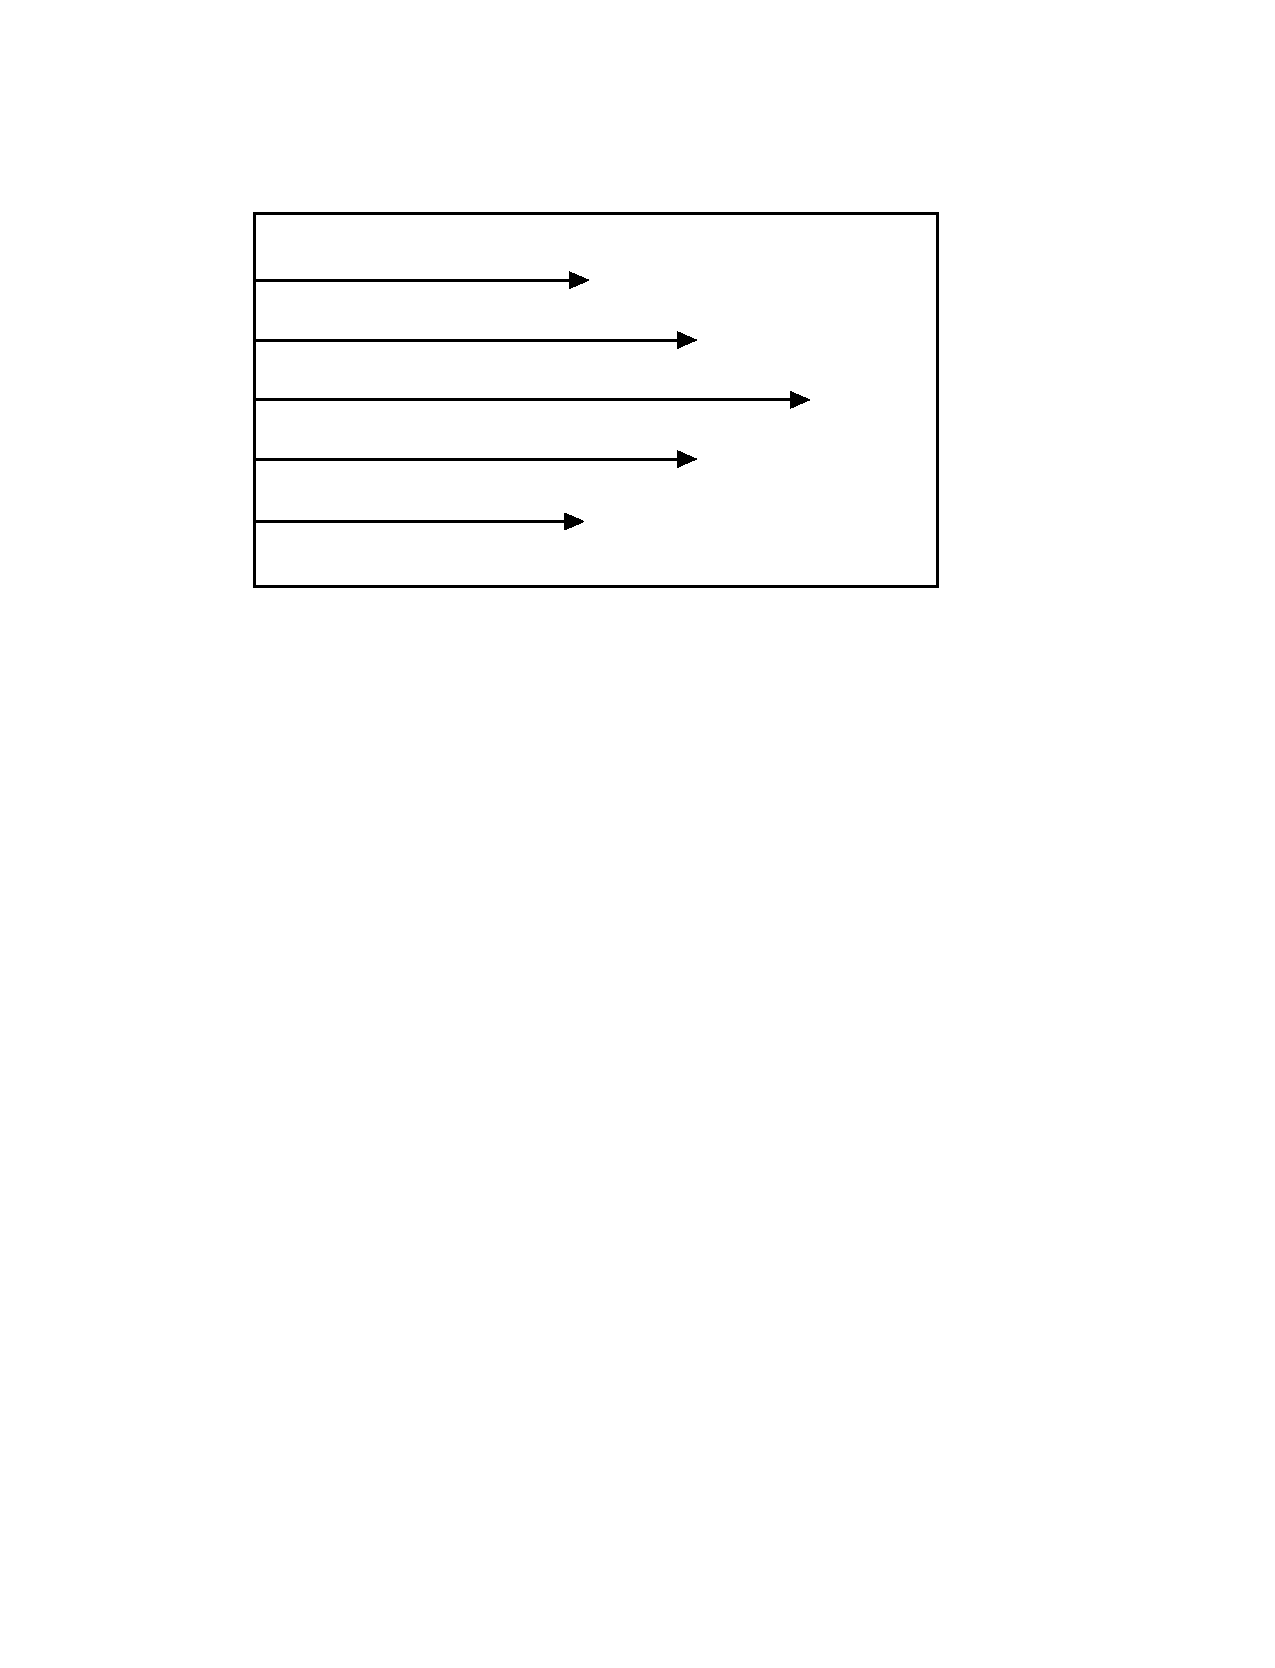
\includegraphics[scale=0.5]{figures/laminar}
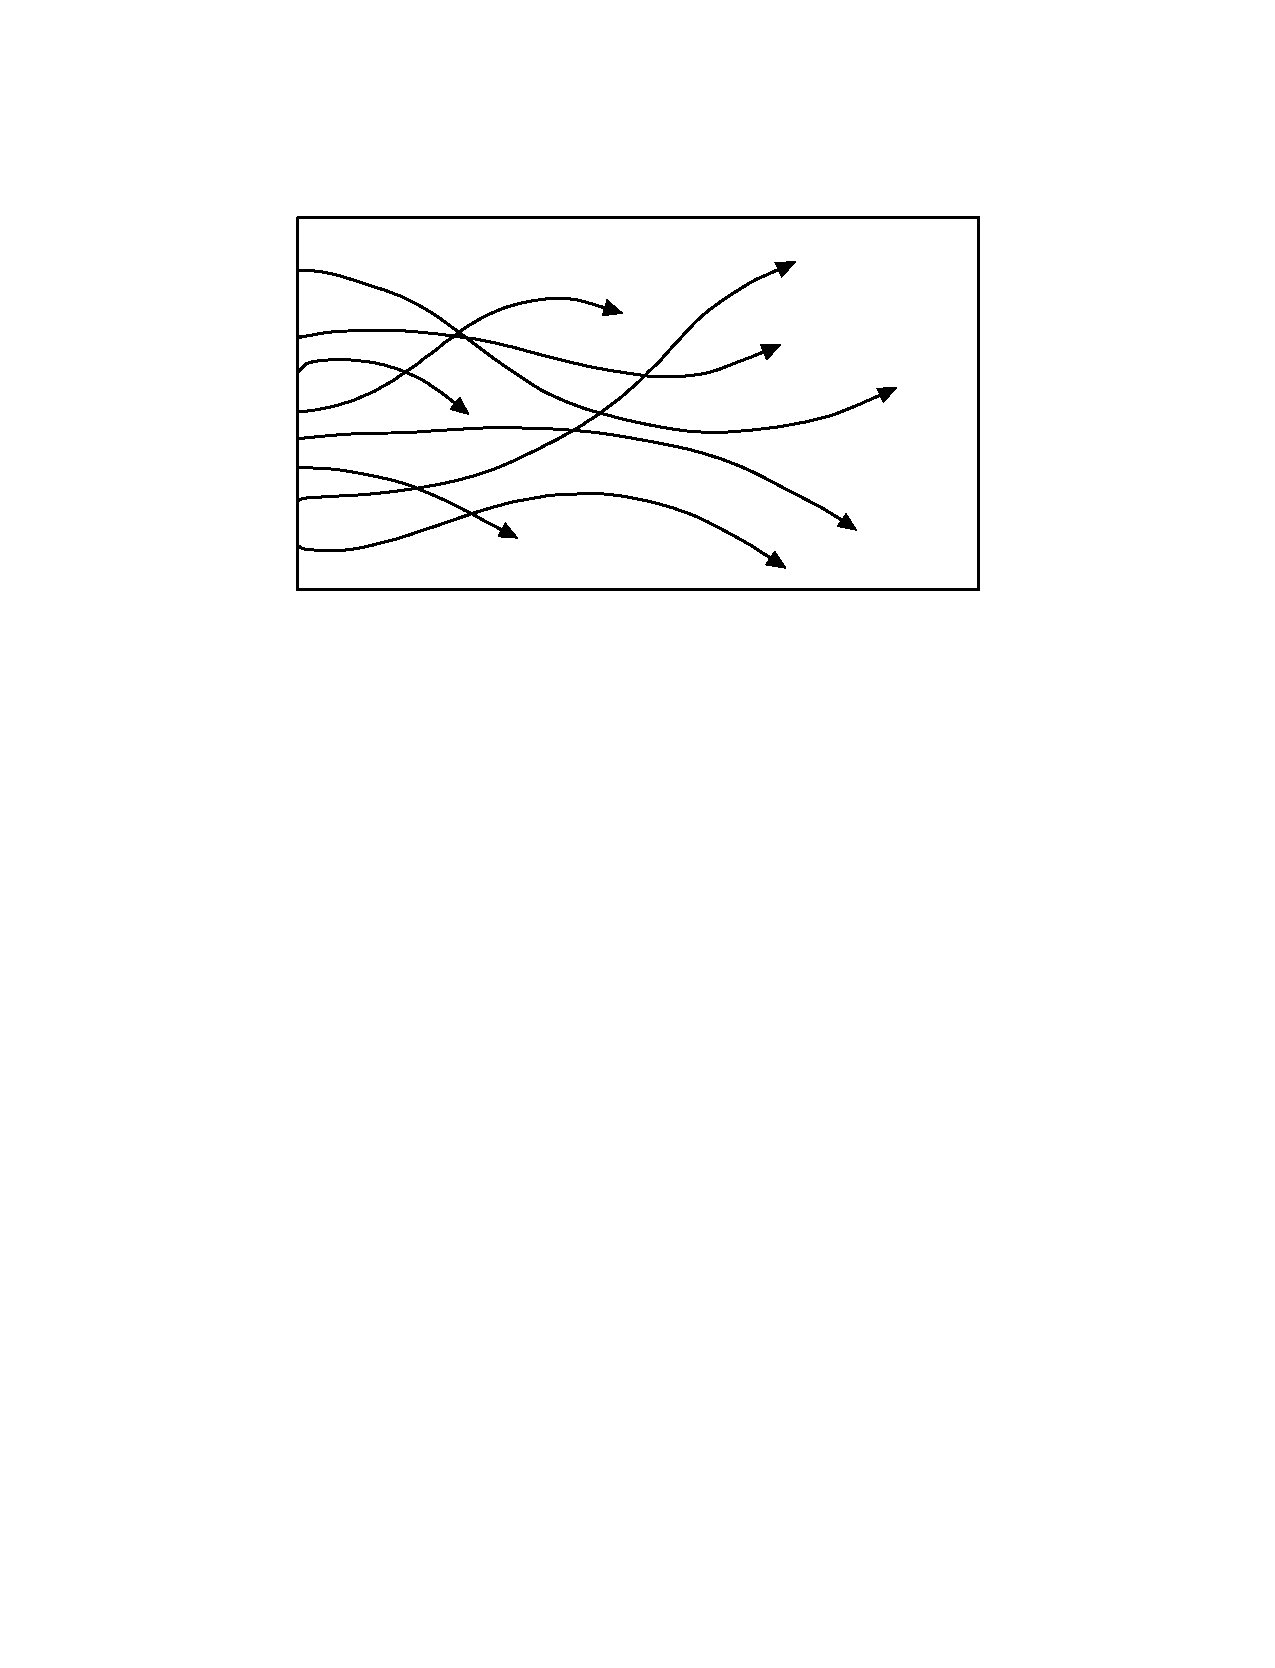
\includegraphics[scale=0.503]{figures/turbulent}
\end{center}
\caption{Example of streamlines in laminar (left) vs. turbulent (right) flow.}
\label{lam_vs_turb}
\end{figure}

The Reynolds number is a dimensionless value that can be used to distinguish laminar flow from turbulent flow. It is defined as follows:
\begin{equation}
\label{Reynolds_num}
\text{Re} = \frac{\rho u L}{\mu}
\end{equation}

\noindent where $\rho$ and $\mu$ are the density and dynamic viscosity of the fluid, respectively, $u$ is the flow velocity, and $L$ is a characteristic length scale associated with the given flow scenario (e.g., pipe diameter). As is demonstrated by the ratio in Equation \eqref{Reynolds_num}, the Reynolds number measures the relative effects of inertial forces compared to viscous forces within a given flow scenario. A small Reynolds number signifies the dominance of viscous forces; fluid parcels moving in tandem want to ``stick together," resulting in the sheared flow and parallel trajectories seen in laminar flow. Turbulence is then characterized by a large Reynolds number, where inertial forces take precedence. Here, deviations within the laminar flow field result in lateral mixing between shear layers. This creates eddies and random trajectories that result in the chaotic motion of turbulent flow. 

This work focuses on the turbulent round jet and its associated dynamics in the context of supercritical fluids. The remainder of this section details a brief overview of important turbulence concepts and numerical methods developed for studying turbulence in order to motivate the modeling and numerical choices made within this work.

\subsection{Mathematics of Turbulence}
Turbulence has been recognized and investigated by scholars in some way, shape, or form for thousands of years; Lucretius being one of the earliest, describing eddy motion in his \textit{De rerum natura} \cite{Benzi:2010}. In that time, a comprehensive theory of turbulence has still not been reached. There are, however, many widely accepted hypotheses and models that at least in part explain certain aspects of turbulent flows.  

Turbulent motion contains a wide range of scales. Richardson formalized this concept by describing turbulence as a compositions of eddies, each with their own characteristic size and velocity \cite{}. From this perspective, large eddies are said to be unstable and break up into smaller eddies, transferring energy down the line to smaller and smaller eddies. This energy cascade continues down to the molecular level where it is dissipated through molecular viscosity. Kolmogorov further developed this theory, noting that for sufficiently high Reynolds flow, the statistics of these smallest-scale motions are uniquely determined by the kinematic viscosity of the fluid, $\nu$, and the dissipation rate, $\varepsilon$ \cite{}. These smallest eddy length, velocity, and time scales at which dissipation occurs, known as the Kolmogorov scales, are defined as follows:
\begin{equation}\label{Kolmogorov}
\begin{aligned}
\eta &\equiv \left(  \nu^3/\varepsilon \right)^{1/4}, \\
u_{\eta} &\equiv \left(  \nu \varepsilon \right)^{1/4}, \\
\tau_{\eta} &\equiv \left(  \nu/ \varepsilon \right)^{1/2} 
\end{aligned}
\end{equation}
While the continuum description introduced in the previous section is still valid for turbulent flows, this vast scale separation and the random nature of fluctuations across these scales, including a dependence on problem-specific flow configurations and boundary conditions, make universal solutions to these types of problems unattainable. To that end, numerical simulations are invaluable in studying turbulence phenomena. 

% \subsubsection{Kolmogorov Scales}
%
%\subsubsection{Reynolds Decomposition}
%
%\subsubsection{Favre Averaging}
%
%\subsubsection{Self-Similarity}


\subsection{Numerical Approaches to Turbulence Modeling}
A vast array of numerical approaches have been developed to tackle the modeling challenges inherent to turbulence, with further development of these and new techniques remaining an active field of research today. We will briefly look at three families of numerical simulation methods in order to highlight the challenges associated with the large scale disparity included in turbulent flows. Methods of note include use of the Reynolds-Averaged Navier-Stokes (RANS) equations, direct numerical simulation (DNS), and large eddy simulation (LES), with scale coverage of each outlined in Figure \ref{DNSvsLESvsRANS}. 
\begin{figure}[h!]
\begin{center}
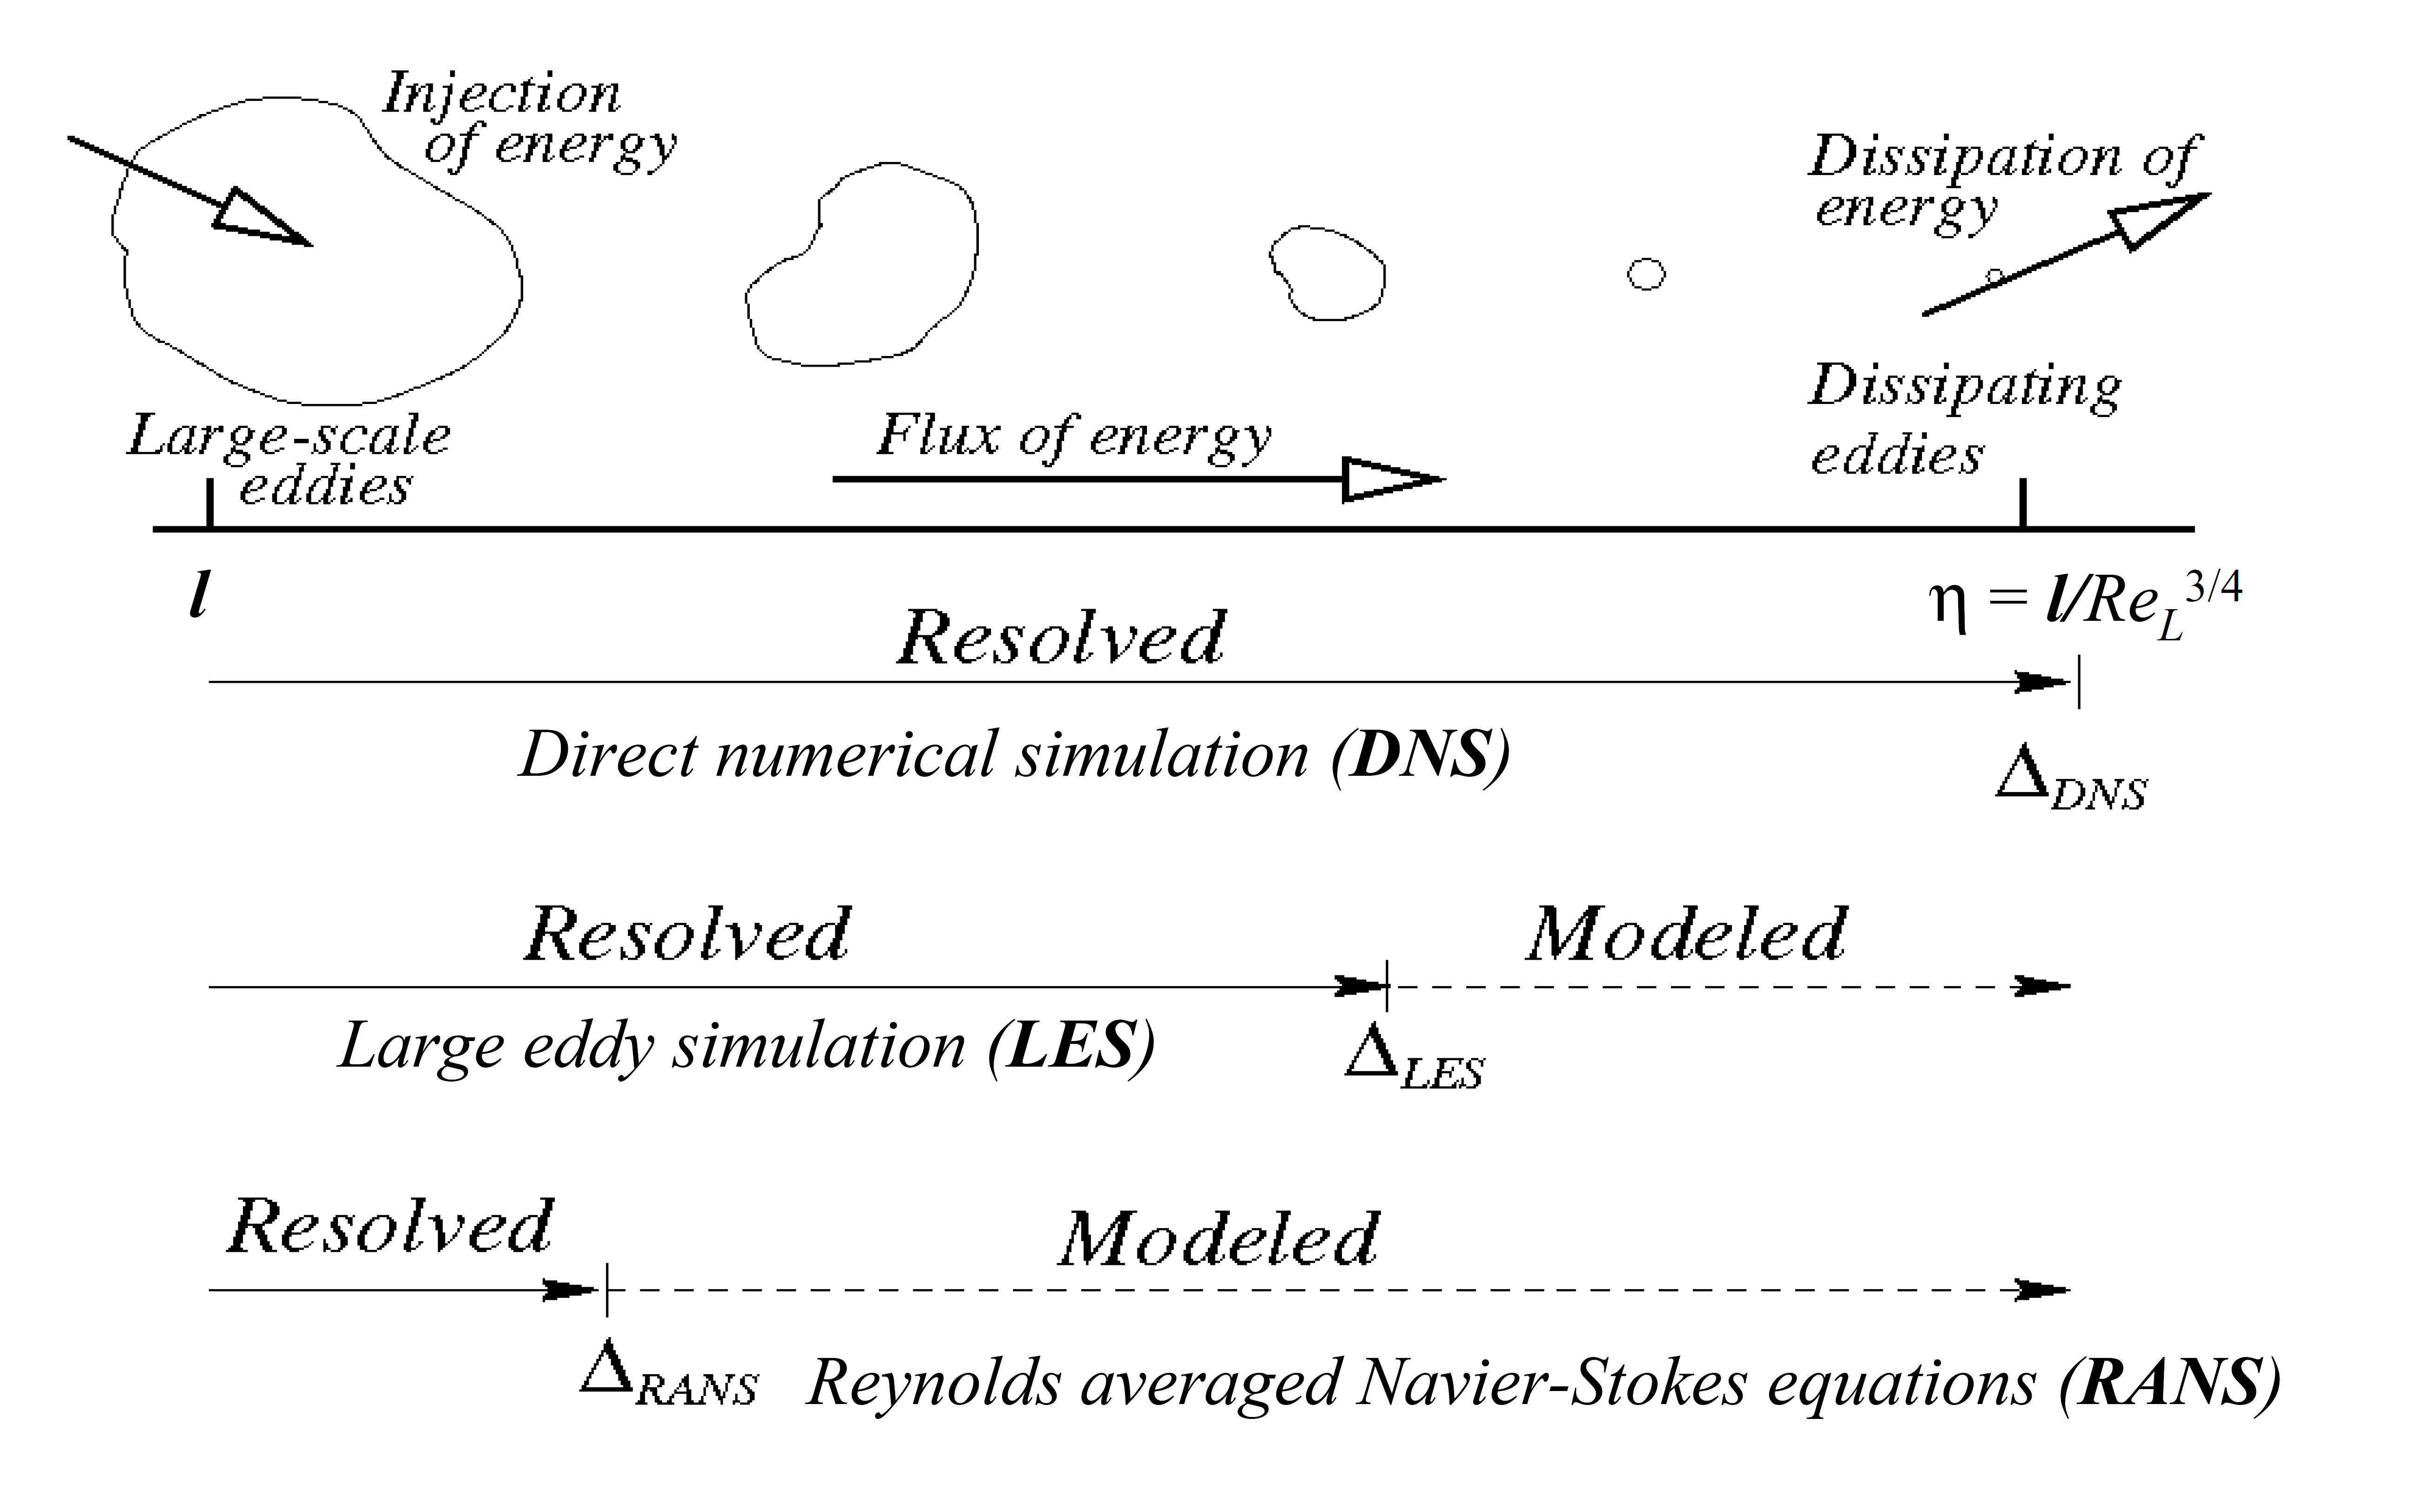
\includegraphics[scale=0.065]{figures/DNSvsLESvsRANS}
\end{center}
\caption{Depiction of the energy cascade present in turbulence along associated scales. Resolved vs. Modeled scales are mapped for \gls{dns}, \gls{les}, and \gls{rans} \cite{}.}
\label{DNSvsLESvsRANS}
\end{figure}

At one extreme, we have \gls{dns}. The aim of \gls{dns} to resolve all scales within the turbulent flow, from the largest eddies down to the Kolmogorov scale. To do this, all components of the Navier-Stokes equations are discretized and numerically advanced. Numerical methods may include high-order finite differencing or pseudo-spectral methods depending on the type of turbulence, flow configuration, and boundary conditions at hand. While \gls{dns} can capture physics across all scales of the flow with high accuracy, this comes at a steep computational cost. Grid spacing and time stepping are highly dependent upon the Reynolds number (approximately as $Re^3$ \cite{Pope}). Thus \gls{dns} very quickly becomes limited to lower Reynolds flows, even with high computing resources. 

On the other end of the spectrum, we have \gls{rans} modeling. The RANS equations make use of the Reynolds decomposition of the flow, in which a random velocity field $\vb{u}$ can be split into an ensemble average, $\langle \vb{u}\rangle$, and a fluctuating component, $\vb{u}'$, such that: 
\begin{equation}\label{rey_decomp}
\begin{aligned}
\vb{u}'(\vb{x},t) & \equiv \vb{u}(\vb{x}, t) - \langle \vb{u}(\vb{x}, t)\rangle, \\
\langle \vb{u}(\vb{x},t)\rangle & = \lim_{N \to \infty}\dfrac{1}{N} \sum\limits_{i=1}^{N} \vb{u}_i(\vb{x}, t)
\end{aligned}
\end{equation}   
where $i$ is the $i-th$ realization of a flow of identical conditions with the number of realizations $N$ tending toward infinity. In practice, for numerical models with the \gls{rans} equations, this is implemented via time averaging: 
$$\langle \vb{u}(\vb{x}, t) \rangle \approx \overbar{\vb{u}(\vb{x})} \equiv \dfrac{1}{T} \int\limits_{t_0}^{t_0+T} \vb{u}(\vb{x}, s) ds$$
where $T$ is taken to be much larger than the time scale of the fluctuating components. By substituting $\vb{u}(\vb{x},t) = \overbar{\vb{u}(\vb{x})} + \vb{u}'(\vb{x}, t)$ particular substitution into the Navier-Stokes equations, one can get a statistical description of the average flow field for the turbulent system (note - the more general decomposition given in equation \eqref{rey_decomp} can be used in the substitution as well to take into consideration a moving average within the flow field. For many of the applications in which \gls{rans} is used, it is enough to look at the steady state given by the time averaged system). Further equations are then needed to model the additional stresses that arise from the nonlinear interactions between components of the mean flow field. Overall, simulations of the \gls{rans} equations resolve the larger scale motions associated with the average motion of the field in a statistical description of the system while the influence of fluctuating fields are incorporated via modeling. While this reduces the computational cost of the numerics, more closure issues arise from the modeling requirements introduced, which present a whole new set of choices and assumptions that are highly problem specific. 

Finally, we have \gls{les}, which falls between the two extremes of the methodology spectrum presented thus far. The strategy with \gls{les} is to only resolve the energy containing scales in the system and model the influence of the smaller scales, as demonstrated in Figure \ref{LES_grid}. This allows for some relaxation in computational cost compared to \gls{dns} without introducing the same degree of modeling assumptions required for \gls{rans}. While still fairly computationally expensive overall, \gls{les} can resolve more of the instantaneous flow field and capture certain physics that inherently depend on the small scale dynamics; quantities of this nature are lost or become highly model dependent in \gls{rans} which introduces more error to the simulation. 

\begin{figure}[h!]
\begin{center}
\begin{tikzpicture}
%% Grid
\draw[step=1cm,black,thin] (0,0) grid (4,4);
%% Arrows for eddy flow
\path[draw,-{Latex[scale=1.5]},use Hobby shortcut,closed=false]
(.2,3.5) .. (.75,3.5);
\path[draw,-{Latex[scale=1.5]},use Hobby shortcut,closed=false]
(1.2,3.5) .. (1.75,3.5);
\path[draw,-{Latex[scale=1.5]},use Hobby shortcut,closed=false]
(2.2,3.5) .. (2.75,3.5);
\path[draw,-{Latex[scale=1.5]},use Hobby shortcut,closed=false]
(3.5,3.8) .. (3.5,3.25);
\path[draw,-{Latex[scale=1.5]},use Hobby shortcut,closed=false]
(3.5,2.8) .. (3.5,2.25);
\path[draw,-{Latex[scale=1.5]},use Hobby shortcut,closed=false]
(3.5,1.8) .. (3.5,1.25);
\path[draw,-{Latex[scale=1.5]},use Hobby shortcut,closed=false]
(3.8,.5) .. (3.25,.5);
\path[draw,-{Latex[scale=1.5]},use Hobby shortcut,closed=false]
(2.8,.5) .. (2.25,.5);
\path[draw,-{Latex[scale=1.5]},use Hobby shortcut,closed=false]
(1.8,.5) .. (1.25,.5);
\path[draw,-{Latex[scale=1.5]},use Hobby shortcut,closed=false]
(.5,.2) .. (.5,.75);
\path[draw,-{Latex[scale=1.5]},use Hobby shortcut,closed=false]
(.5,1.2) .. (.5,1.75);
\path[draw,-{Latex[scale=1.5]},use Hobby shortcut,closed=false]
(.5,2.2) .. (.5,2.75);

%% Grid
\draw[step=1cm,black,thin] (5,0) grid (9,4);
%% Arrows for smaller eddy flow
\path[draw,-{Latex[scale=1.5]},use Hobby shortcut,closed=false]
(6.5,2.2) .. (6.5,2.75);
\path[draw,-{Latex[scale=1.5]},use Hobby shortcut,closed=false]
(7.2,2.5) .. (7.75,2.5);
\path[draw,-{Latex[scale=1.5]},use Hobby shortcut,closed=false]
(7.5,1.75) .. (7.5,1.2);
\path[draw,-{Latex[scale=1.5]},use Hobby shortcut,closed=false]
(6.75,1.5) .. (6.2,1.5);

%% Grid
\draw[step=1cm,black,thin] (10,0) grid (14,4);
%% Arrows for smaller eddy flow
\path[draw=red,-{Latex[scale=1.5]},use Hobby shortcut,closed=false]
(11.25,2.85) .. (11.75,2.85);
\path[draw=red,-{Latex[scale=1.5]},use Hobby shortcut,closed=false]
(11.85,2.75) .. (11.85,2.25);
\path[draw=red,-{Latex[scale=1.5]},use Hobby shortcut,closed=false]
(11.75,2.15) .. (11.25,2.15);
\path[draw=red,-{Latex[scale=1.5]},use Hobby shortcut,closed=false]
(11.15,2.25) .. (11.15,2.75);
\end{tikzpicture}
\end{center}
\caption{LES resolves large scale eddies (black) and models the effects of fine scale eddies (red) that are unresolved due to mesh size.}
\label{LES_grid}
\end{figure}
The procedure for \gls{les} involves decomposing random velocity field $\vb{u}$ into filtered components, $\overline{\vb{u}}$, and residual components, $\vb{u}''$, such that: 
\begin{equation} \label{les_filtering}
\begin{aligned}
\vb{u}''(\vb{x},t) & \equiv \vb{u}(\vb{x}, t) - \overline{\vb{u}(\vb{x}, t)}, \\
\overline{\vb{u}(\vb{x},t)} & =  \int\limits_{-\infty}^{\infty}\int\limits_{-\infty}^{\infty} \vb{u}(\vb{r},s)G(\vb{x-r}, t-s) d\vb{r}ds
\end{aligned}
\end{equation}
$G$ is the convolution kernel of associated filter spatial and/or temporal cutoff $\Delta$ and $\tau_c$, respectively, satisfying $\int\limits_{-\infty}^{\infty}\int\limits_{-\infty}^{\infty}G(\vb{r}, s) d\vb{r}ds = 1$. In practice, common kernels are only spatially dependent. Applying this filtering procedure to the Navier-Stokes equations yields an additional term known as the residual stress tensor that must be modeled. The filtered Navier-Stokes equations can then be discretized to numerically simulate the large eddy behavior of the system.

This general \gls{les} procedure may seem similar to what was described for the \gls{rans} model, especially in terms of the decomposition of the flow field, but there are key differences to note. Conceptually, the result of a numerical simulation using \gls{rans} describes an average behavior of turbulent flow over many instances or experiments. The output of these simulations is not a snapshot of one instance of the given flow field but rather an approximation to how the flow behaves in a statistical sense. \gls{les} does approximate a single realization of the flow field, just only including the low frequency modes of the system which contain the majority of the energy. Additionally, the components of the Reynolds decomposition obey the following rules:
\begin{equation*}
\overbar{\overbar{\vb{u}}} = \overbar{\vb{u}}, \quad
\overbar{\vb{u}'} = 0
\end{equation*}
These rules do not hold for $\overline{\vb{u}}$ and $\vb{u}''$:
\begin{equation*}
\overline{\overline{\vb{u}}} \neq \overline{\vb{u}}, \quad
\overline{\vb{u}''} \neq 0
\end{equation*}
We use \gls{les} in this work to balance the computational cost of the simulation with the degree of resolution for physical phenomena within the flow. Many studies involving turbulent supercritical fluids utilize \gls{les}, as will be seen in the next section, with additional research having been conducted regarding appropriate choices in modeling for the residual stress tensor. Model selection and further details on filtering are discussed in Chapter 2. 

%\begin{figure}[h!]
%\begin{center}
%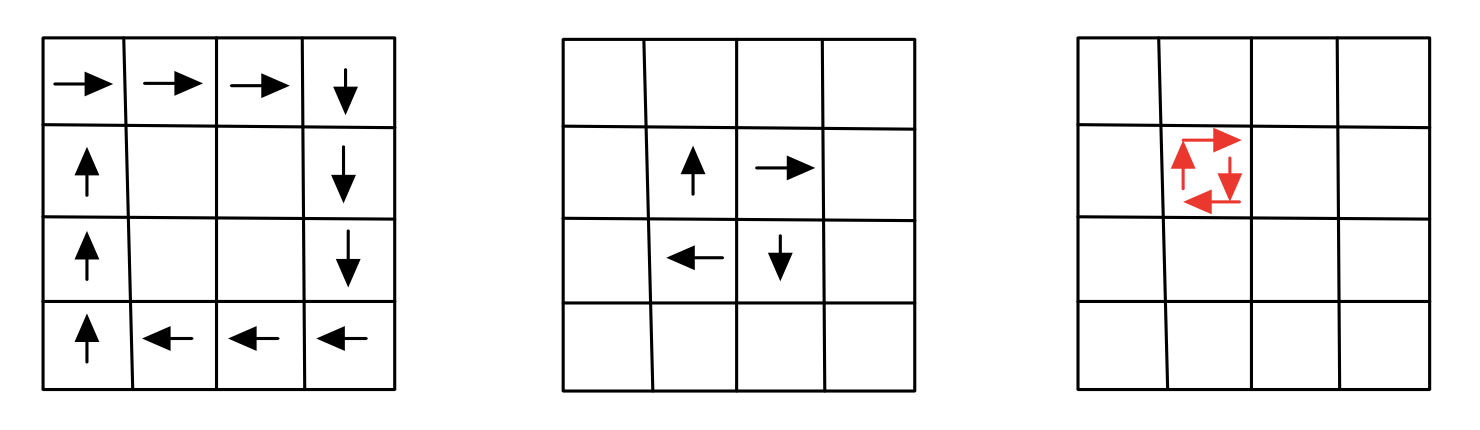
\includegraphics[scale=0.5]{figures/LES_grid}
%\end{center}
%\end{figure}

\section{Current Research Landscape}
Here we provide a brief overview of some of the current trends in research regarding supercritical fluids. Both experimental and numerical works are discussed in order to highlight the challenges associated with studying supercritical fluids and what approaches are common practice in doing so. This is not an exhaustive review by any means, but provides insights into the general landscape for which this work fits in. 
\subsection{Experimental Contributions}
Current experimental research is mainly application oriented. Research into the \gls{sco2} jet's rock breaking ability has been of primary importance to \gls{egs} applications \cite{EGScomp, EGS2, very_rock, experiment, rb}, with additional focus being given to pipeline leakage and flow dynamics upon wall impact \cite{WANG2015210, WANG201977}, which unfortunately does not explore the underlying turbulence statistics of the flow. Enhanced recovery of unconventional reservoirs for oil and gas development is an additional area where rock breaking research is often applied \cite{HUANG2020106735, HUANG2019}. Chemical engineering design aspects of \gls{sco2} injection are more focused on solubility dynamics as opposed to turbulence \cite{freejet, pulse_jet}. Other experiments focus on similar application specific quantities of interest, such as heat transfer and mixing, which is related in part to the turbulence dynamics \cite{heated_cyl, 10.1115/FEDSM2022-87029}, but they also note the difficulty in experimental design for investigating these aspects of the flow under the conditions needed to replicate those in real applications \cite{freejet}. Thus, numerical simulations are necessary to further explore the turbulence statistics of these flows.

\subsection{Numerical Contributions}
Numerical simulations are a necessary tool for investigating many aspects of supercritical flow fields due to the often challenging nature of experiment design for the extreme conditions inherent to these systems. Studies using \gls{dns} have been implemented to help establish benchmark test cases for other types of numerical schemes \cite{OVAIS2022, SENGUPTA2019}. Ruiz et al. use 2D \gls{dns} to simulate a mixing layer created by two streams of supercritical Oxygen and gaseous Nitrogen, using two different \gls{cfd} solvers to add confidence to their results \cite{article}. A 3D \gls{dns} is used by Ries at al. to simulate a round Nitrogen jet for comparison with experimental data produced by Mayer et al. \cite{DNS_N}. However, this study requires a reduction in Reynolds number from $1.62 \times 10^5$, based on the injection diameter, to $5300$ in order to feasibly execute the computations. Li also utilizes a low Reynolds number of $1750$ to study a round turbulent \gls{sco2} jet with a preconditioning scheme \cite{Li2012}. The \gls{rans} approach has also been implemented utilizing theory from the ideal gas case \cite{RANS}, but with the goal of ascertaining a more general understanding of why specifically \gls{sco2}'s rock-breaking ability is better than that of water. 

Much research has gone into the development of appropriate numerical methods for investigations regarding turbulence in supercritical fluids. In order to maintain a high Reynolds flow and better capture the effects of the supercritical nature of the fluid on the turbulence dynamics, the use of \gls{les} has been explored. The impact of \gls{sgs} models in capturing transcritical and supercritical dynamics of cryogenic Nitrogen have been analyzed through comparison with the Mayer et al. experiment and highly accurate \gls{nist} data \cite{PETIT201361, doi:10.1080/00102200500287613, doi:10.1063/1.1795011, doi:10.1063/1.4937948, Same_LES}. Schmitt et al. does a similar investigation using \gls{les}, then extending their investigation to include \gls{sco2} after validation with the Mayer et al. data \cite{LES_N}. However, this investigation uses low-pressure jets and does note the \gls{sgs} models might need additional contributions to handle non-linearities and the pressure regime. While many of these investigations note that \gls{sgs} models may need modification to deal with supercritical flows \cite{LES_N, PETIT201361, doi:10.1063/1.4937948, doi:10.1080/00102200500287613}, it is noted by Muller et al. that given a sufficiently fine grid, the influence of \gls{sgs} modeling and numerical flux discretization is essentially limited to second-order moments \cite{doi:10.1063/1.4937948}. Thus, we will be using the compressible version of the dynamic Smagorinksy \gls{sgs} closures for our investigation, with further consideration of any influence of \gls{sgs} model on our quantities of interest being noted later on. 

Many of the numerical investigations sited thus far consider cryogenic nitrogen in order to compare with the Mayer et al. experiment on supercritical jet turbulence \cite{mayer2003raman}. A wide variety of numerical investigations into jet turbulence using \gls{sco2} exist but typically explore either other parameter regimes of interest or application-specific quantities of interest. Examples of turbulent adjacent quantities of interest include fluctuation characteristics based on inlet conditions \cite{ZHANG2022124125}, effects of nozzle and aperture differences on pressure and velocity decay \cite{en13102627} and wave features \cite{LIU2021108422}, mixing between \gls{sco2} and other fluid phases \cite{RAMAN2018}, and energy dissipation \cite{LI2020103650}. These studies all involve high pressure jets and are commonly found in applications involving rock fracturing. Related configurations are also studied, such as the swirling-round \gls{sco2} jet \cite{en14010106}, turbulent jet-in-crossflows \cite{ZHANG2022}, slot jet impingement \cite{ALKANDARI2022122949}, and channel flow \cite{ROGALEV2020}.

While much of the literature thus far has explored the impact of different numerical methods on modeling supercritical fluid flows and has aimed to strengthen the validity of these simulations in spite of the lack of experimental data available in the current landscape, a general consensus has still not been reached on how the supercritical nature of these fluids impacts the turbulence physics of these models. Thus, there remain open questions for understanding the fundamental flow behavior of turbulent jets in a supercritical environment, especially near the supercritical point, where both experimental and numerical investigations are still a challenge.

Our objective is to use \gls{les} to investigate the turbulence physics of \gls{sco2} near the critical point in order to capture the effects of widely varying thermal properties of supercritical fluids. Using the compressible Navier-Stokes equation solver, \textit{PeleC} \cite{PeleC1, PeleC2}, closed with the \gls{srk}, we consider three cases in order to examine various quantities of interest associated with classical turbulence mechanics. These three cases are chosen to capture different areas around a peak in specific heat that is associated with the pseudo-critical region. The rest of this dissertation is outlined as follows. Chapter 2 details the model used for this study. Chapter 3 gives an overview of the numerical methods implemented through \textit{PeleC}. Chapter 4 outlines the simulation setup with parameter choices and validation. Results for cross-case comparisons and comparisons with external work are then presented in Chapter 5, with a summary and future work detailed in Chapter 6. 





